% !TeX program = xelatex
\documentclass[11pt]{ctexart}
\usepackage[a4paper,margin=1in]{geometry}
\usepackage{amsmath}
\usepackage{amssymb}
\usepackage{booktabs}
\usepackage{graphicx}
\usepackage{float}
\usepackage{xurl}
\usepackage{hyperref}
\usepackage{xcolor}
\usepackage{caption}
\usepackage{subcaption}

\hypersetup{
  colorlinks=true,
  linkcolor=blue,
  urlcolor=blue,
  citecolor=blue
}

\title{Project 1: MNIST Classification with NumPy Neural Networks}
\author{陈博闻 \quad Student ID: 22300130089}
\date{\today}

\newcommand{\githuburl}{https://github.com/lrond/pj1-mnist-numpy}
\newcommand{\checkpointurl}{https://www.modelscope.cn/models/lrond1/pj1-mnist-numpy-checkpoints}

\begin{document}
\maketitle

\begin{abstract}
This report presents a NumPy-only implementation of basic neural-network components for MNIST handwritten digit classification. I implemented the linear layer forward and backward passes, softmax cross-entropy, a 2D convolution operator, max pooling, MLP and CNN models, SGD, momentum gradient descent, and learning-rate schedulers. The MLP baseline reaches 94.59\% test accuracy. Under a fair momentum-based training setting, the MLP reaches 96.80\% test accuracy, while the CNN reaches 98.46\% test accuracy. I further study optimization and error analysis with visualizations.
\end{abstract}

\section*{Submission Links}
\begin{itemize}
  \item Code repository: \url{\githuburl}
  \item Trained checkpoints: \url{\checkpointurl}
\end{itemize}
The GitHub repository excludes the MNIST dataset, trained weights, and large generated artifacts, following the project instructions.

\section{MLP Baseline}

\subsection{Implemented Operators}
For a mini-batch input $X \in \mathbb{R}^{N \times d_{\text{in}}}$, the linear layer computes
\[
Y = XW + b.
\]
Given the upstream gradient $G = \frac{\partial L}{\partial Y}$, the backward pass computes
\[
\frac{\partial L}{\partial W}=X^\top G,\quad
\frac{\partial L}{\partial b}=\sum_{i=1}^{N} G_i,\quad
\frac{\partial L}{\partial X}=GW^\top.
\]
The softmax cross-entropy loss is
\[
L=-\frac{1}{N}\sum_{i=1}^{N}\log
\frac{\exp z_{i,y_i}}{\sum_c \exp z_{i,c}},
\]
implemented with max-shifted logits for numerical stability.

\subsection{Model and Training}
The baseline MLP uses the architecture
\[
784 \rightarrow 256 \rightarrow 10,
\]
with ReLU activation after the hidden layer. The training set is split into 50,000 training images and 10,000 validation images using a fixed random seed. Images are normalized to $[0,1]$.

The baseline is trained for 5 epochs with batch size 64, SGD, initial learning rate 0.06, and MultiStepLR milestones at 800, 2400, and 4000 iterations.

\begin{figure}[H]
  \centering
  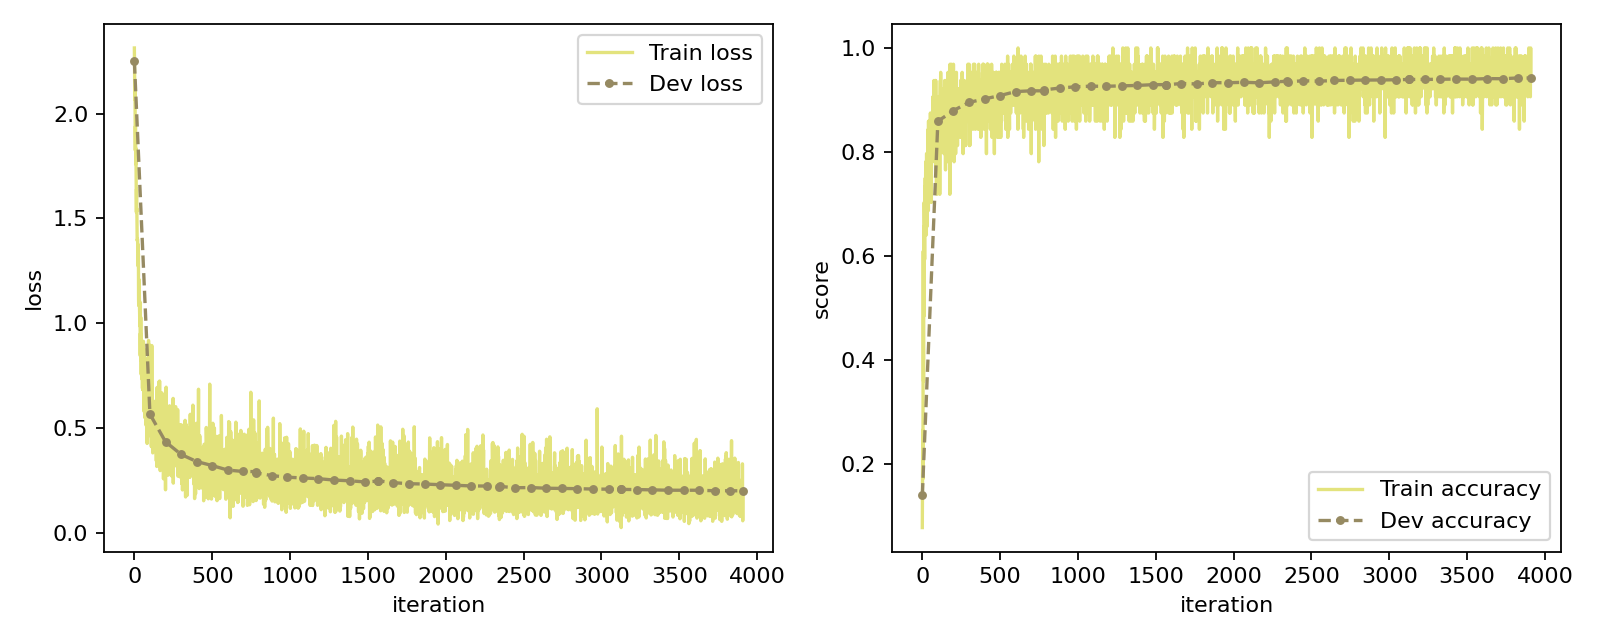
\includegraphics[width=0.92\linewidth]{figures/mlp_baseline_curve.png}
  \caption{MLP baseline training and validation curves.}
\end{figure}

\section{CNN Model and MLP-vs-CNN Comparison}

\subsection{CNN Implementation}
The convolution operator is implemented from scratch. For each image patch $P_{n,h,w}$ and filter $W_o$, the output is
\[
Y_{n,o,h,w} = \sum_{c,r,s} P_{n,c,h,w,r,s} W_{o,c,r,s} + b_o.
\]
The implementation uses NumPy sliding windows only to extract image patches; the convolution, gradients, and parameter updates are implemented manually with NumPy tensor operations. I also implemented max pooling and its backward pass, routing gradients to the maximum locations in each pooling window.

The final CNN architecture is
\[
\text{Conv2D}(1,16,3) \rightarrow \text{ReLU} \rightarrow \text{MaxPool2D}(2)
\rightarrow \text{Flatten} \rightarrow 128 \rightarrow \text{ReLU} \rightarrow 10.
\]

\subsection{Fair Comparison}
To compare the MLP and CNN under similar training conditions, both models are trained for 5 epochs with batch size 64, momentum gradient descent, initial learning rate 0.02, and the same MultiStepLR milestones.

\begin{table}[H]
\centering
\caption{Main MNIST results.}
\small
\begin{tabular}{lcccc}
\toprule
Experiment & Optimizer & Epochs & Best val. acc. & Test acc. \\
\midrule
MLP baseline & SGD + MultiStepLR & 5 & 0.9424 & 0.9459 \\
MLP fair setting & Momentum + MultiStepLR & 5 & 0.9657 & 0.9680 \\
CNN fair setting & Momentum + MultiStepLR & 5 & 0.9855 & 0.9846 \\
\bottomrule
\end{tabular}
\end{table}

\begin{figure}[H]
  \centering
  \begin{subfigure}{0.48\linewidth}
    \centering
    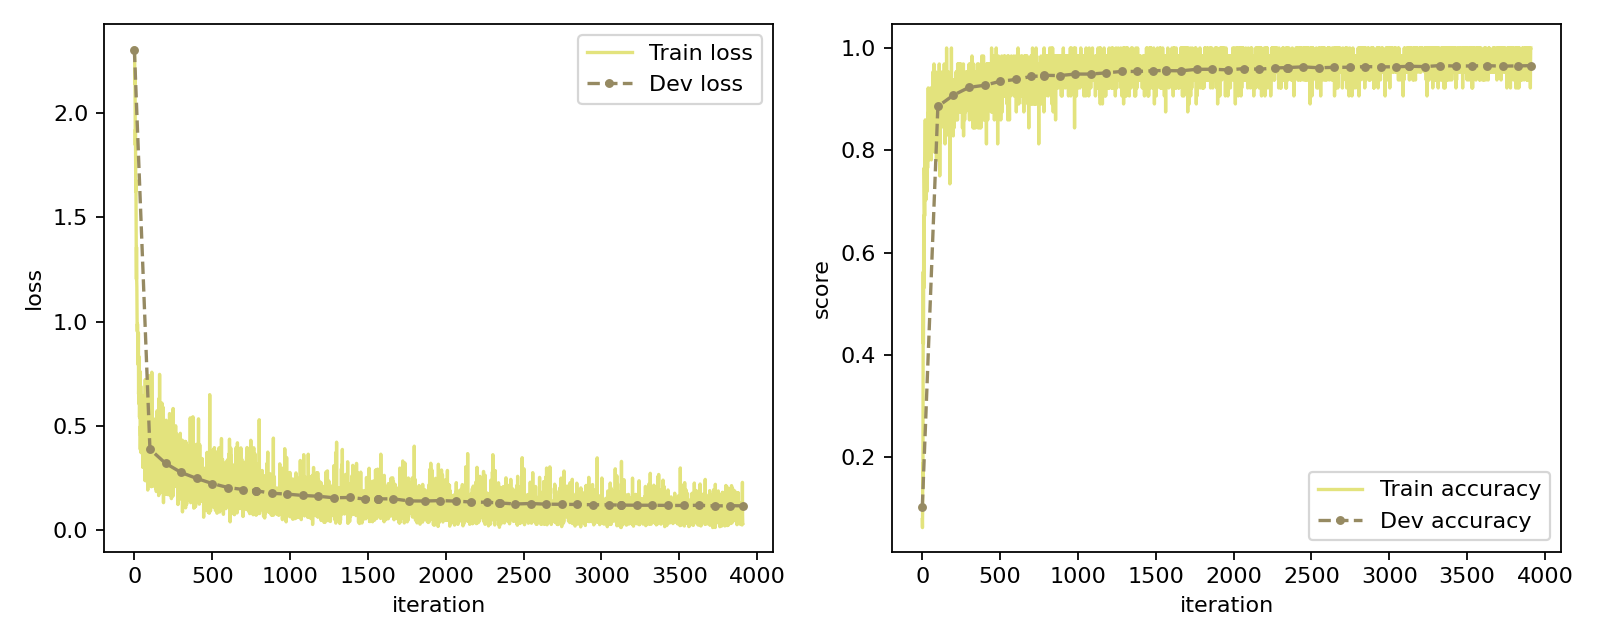
\includegraphics[width=\linewidth]{figures/mlp_momentum_curve.png}
    \caption{MLP fair setting}
  \end{subfigure}
  \begin{subfigure}{0.48\linewidth}
    \centering
    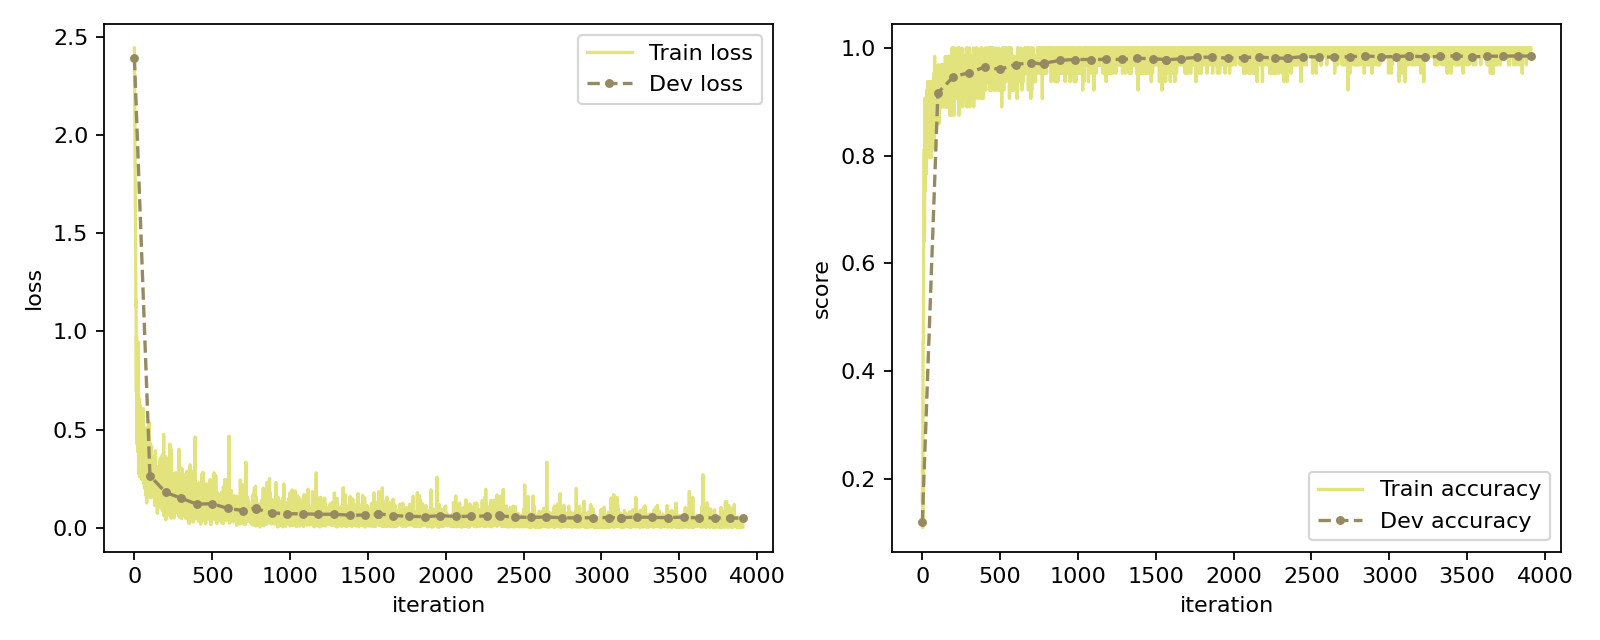
\includegraphics[width=\linewidth]{figures/cnn_momentum_curve.png}
    \caption{CNN fair setting}
  \end{subfigure}
  \caption{Fair MLP-vs-CNN comparison under the same optimizer family, batch size, epoch count, and scheduler.}
\end{figure}

The CNN performs better than the MLP in both validation and test accuracy. This matches the expected inductive bias: handwritten digits contain local stroke patterns and spatial structure. The convolution layer shares filters across image locations, making it easier to learn translation-tolerant local features. Max pooling further reduces sensitivity to small shifts. In contrast, the MLP treats each pixel position as an independent input dimension and has to learn spatial patterns from fully connected weights.

\section{Additional Direction 1: Optimization}

I studied momentum as an optimization modification. To isolate the effect of momentum, I compared two MLPs with the same architecture, same initial learning rate 0.02, same batch size, same 5 epochs, and the same MultiStepLR schedule. The only changed factor is the optimizer.

\begin{table}[H]
\centering
\caption{Optimization comparison with only the optimizer changed.}
\begin{tabular}{lccc}
\toprule
Experiment & Initial LR & Best validation accuracy & Test accuracy \\
\midrule
SGD + MultiStepLR & 0.02 & 0.9203 & 0.9238 \\
Momentum + MultiStepLR & 0.02 & 0.9657 & 0.9680 \\
\bottomrule
\end{tabular}
\end{table}

\begin{figure}[H]
  \centering
  \begin{subfigure}{0.48\linewidth}
    \centering
    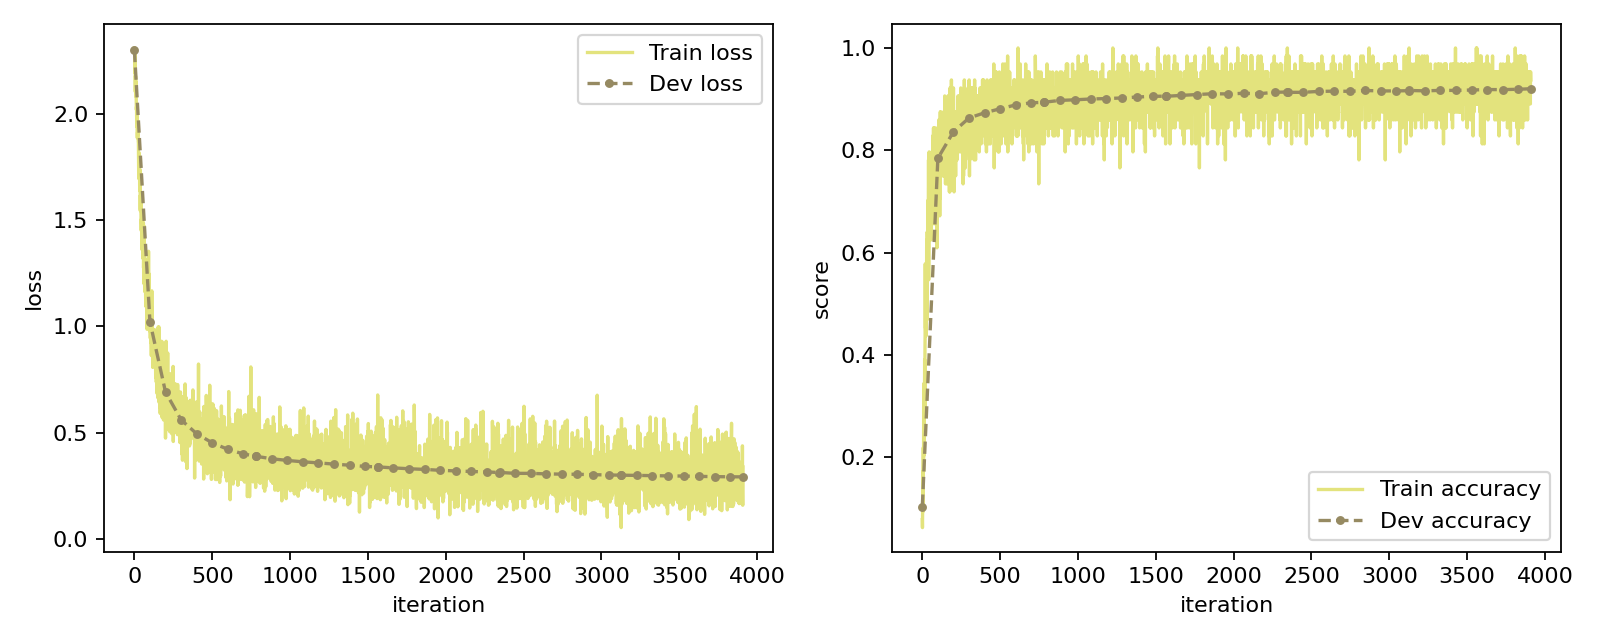
\includegraphics[width=\linewidth]{figures/mlp_sgd_lr002_curve.png}
    \caption{SGD}
  \end{subfigure}
  \begin{subfigure}{0.48\linewidth}
    \centering
    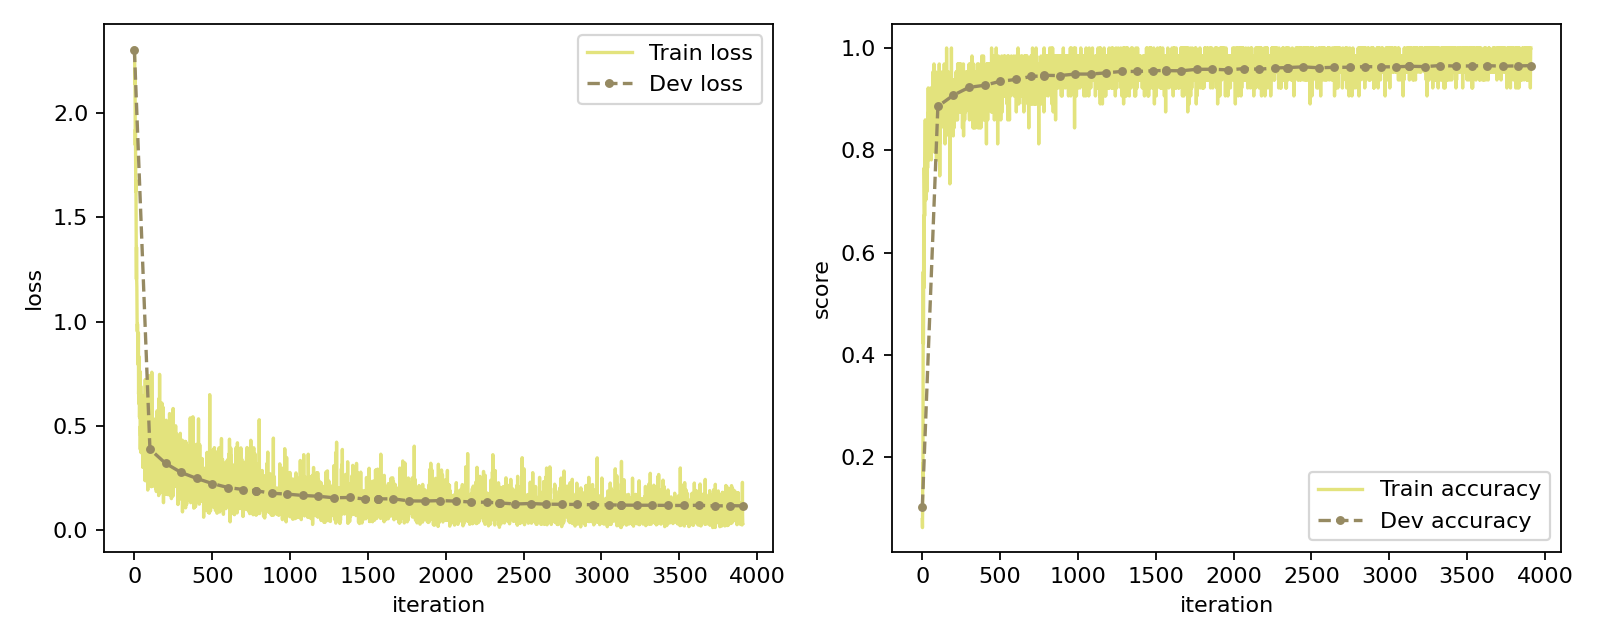
\includegraphics[width=\linewidth]{figures/mlp_momentum_curve.png}
    \caption{Momentum}
  \end{subfigure}
  \caption{Optimization comparison for the MLP.}
\end{figure}

Momentum improves convergence substantially. It accumulates a velocity term, which helps continue updates along consistent descent directions and reduces oscillation in noisy mini-batch gradients. Under the same learning rate and schedule, momentum improves test accuracy from 92.38\% to 96.80\%.

\section{Additional Direction 2: Error Analysis and Visualization}

\subsection{Confusion Matrices}
The MLP baseline and final CNN confusion matrices are shown below. The MLP baseline most often confuses visually similar pairs such as $9\rightarrow4$, $5\rightarrow3$, $7\rightarrow2$, $4\rightarrow9$, and $2\rightarrow8$. The CNN reduces most of these errors; its remaining mistakes are concentrated on ambiguous handwriting such as $9\rightarrow7$, $7\rightarrow2$, and $5\rightarrow3$.

\begin{figure}[H]
  \centering
  \begin{subfigure}{0.48\linewidth}
    \centering
    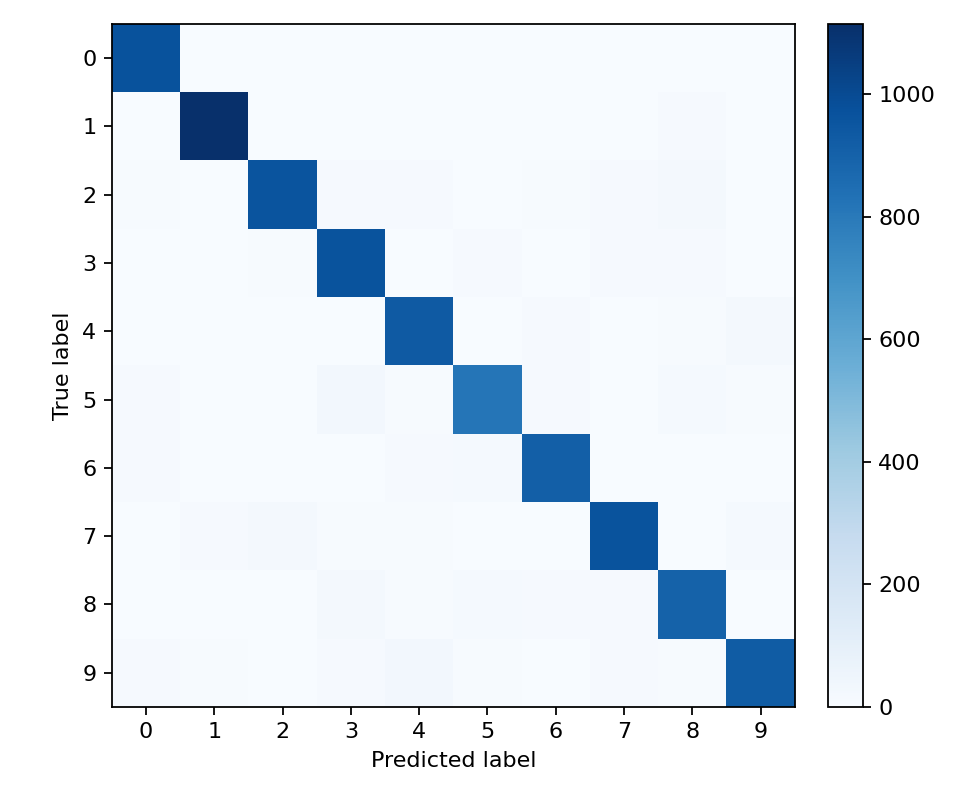
\includegraphics[width=\linewidth]{figures/mlp_confusion_matrix.png}
    \caption{MLP baseline}
  \end{subfigure}
  \begin{subfigure}{0.48\linewidth}
    \centering
    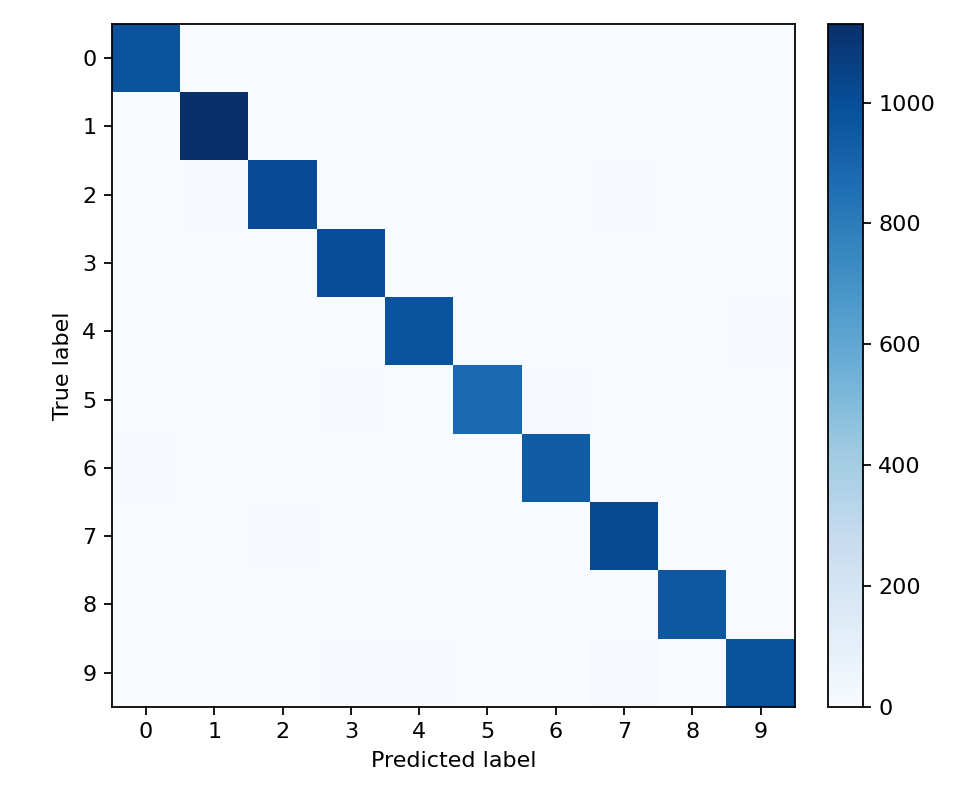
\includegraphics[width=\linewidth]{figures/cnn_confusion_matrix.png}
    \caption{CNN}
  \end{subfigure}
  \caption{Confusion matrices on the MNIST test set.}
\end{figure}

\subsection{Misclassified Examples}
The misclassified examples show that many remaining errors are understandable even for humans: some digits have weak strokes, unusual writing styles, or shapes that resemble another class. For example, $4$ and $9$ share a loop-and-stem structure, while $3$, $5$, and $8$ can look similar when strokes are connected or missing.

\begin{figure}[H]
  \centering
  \begin{subfigure}{0.48\linewidth}
    \centering
    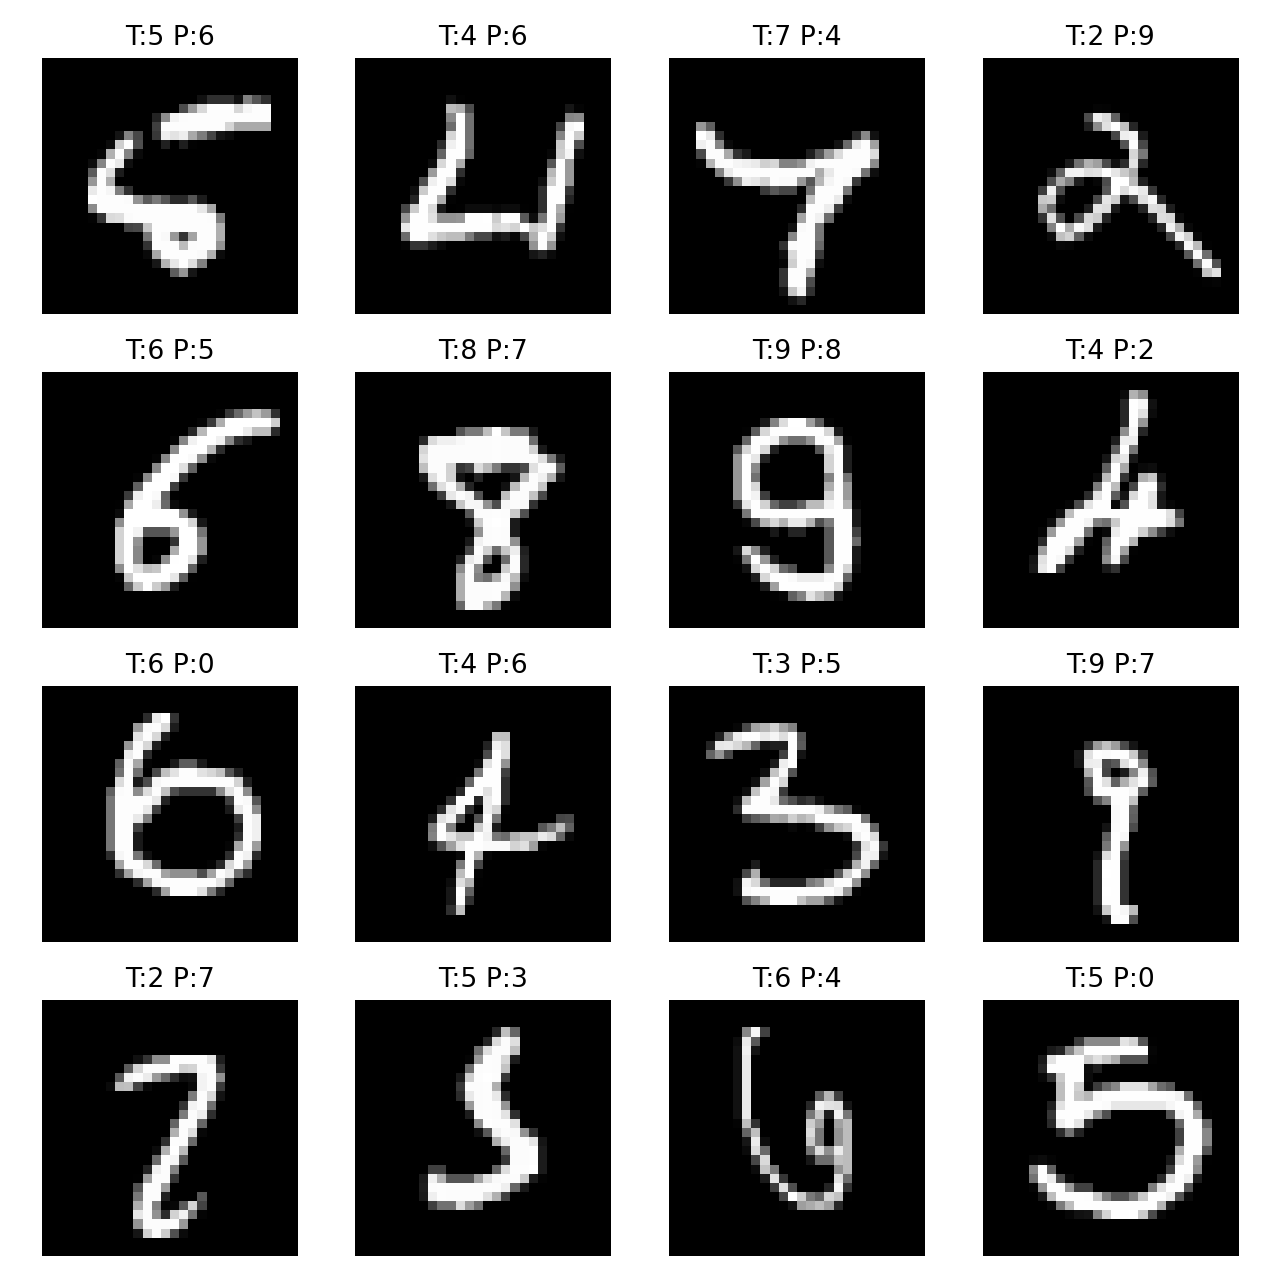
\includegraphics[width=\linewidth]{figures/mlp_misclassified.png}
    \caption{MLP baseline}
  \end{subfigure}
  \begin{subfigure}{0.48\linewidth}
    \centering
    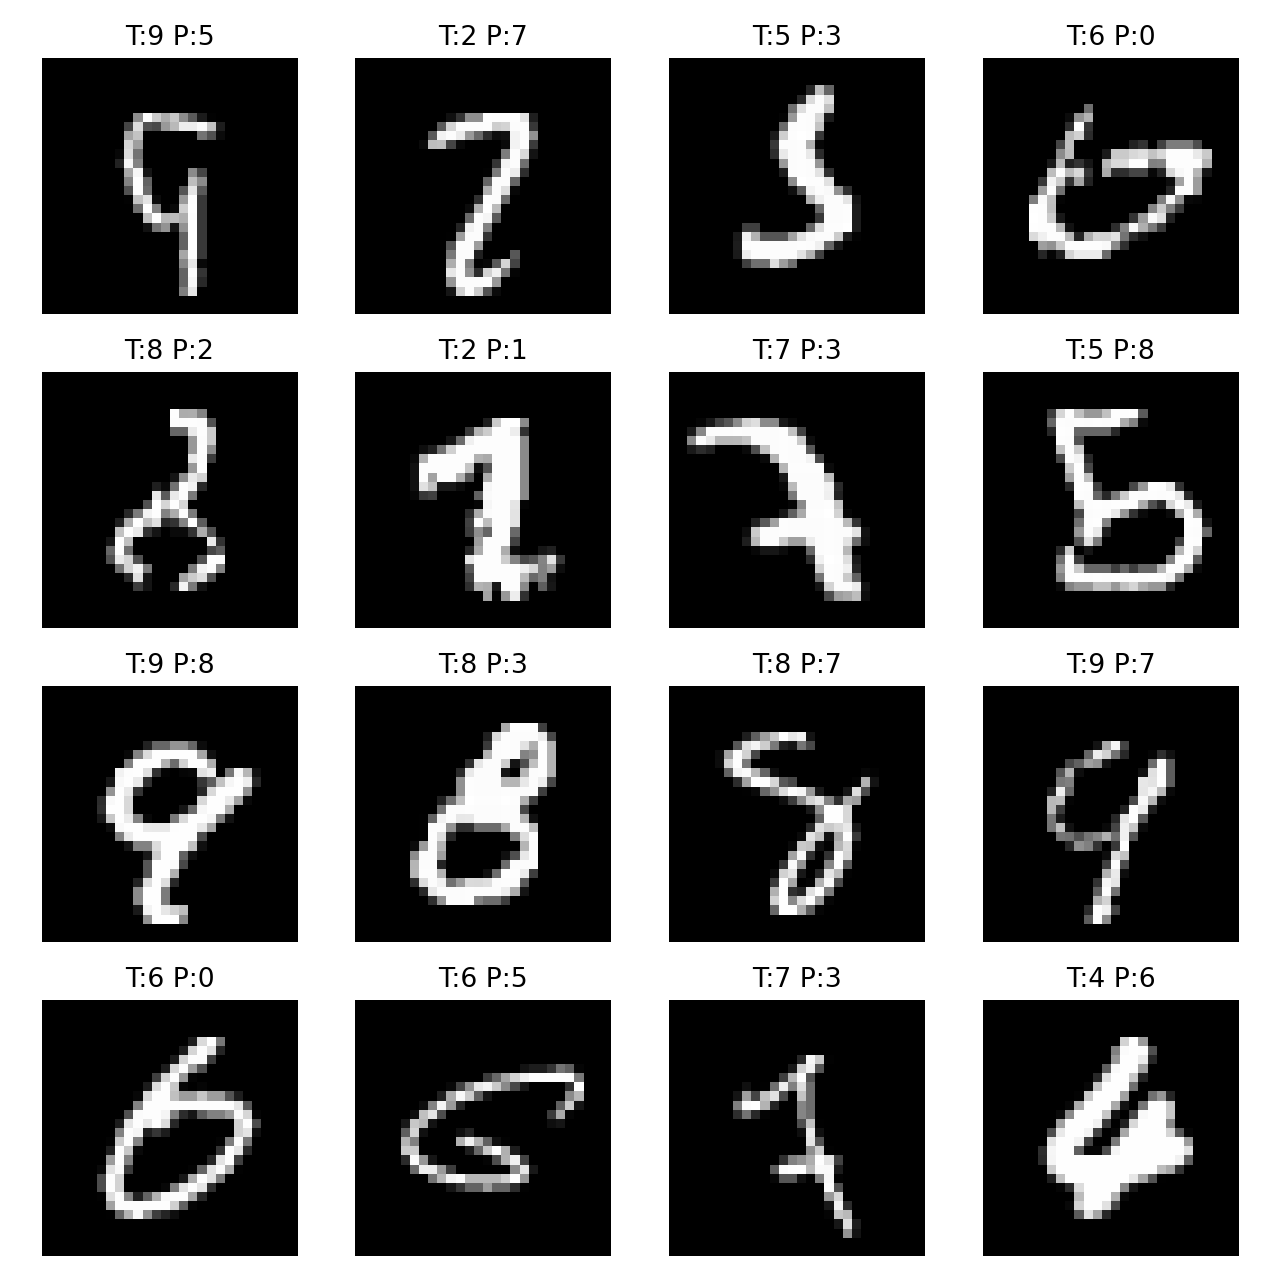
\includegraphics[width=\linewidth]{figures/cnn_misclassified.png}
    \caption{CNN}
  \end{subfigure}
  \caption{Misclassified test examples. Titles show true and predicted labels.}
\end{figure}

\subsection{Weights and Kernels}
The MLP first-layer weights can be reshaped into $28\times28$ templates. These templates capture coarse global pixel patterns. The CNN kernels instead learn local stroke detectors, which is more suitable for digit images.

\begin{figure}[H]
  \centering
  \begin{subfigure}{0.48\linewidth}
    \centering
    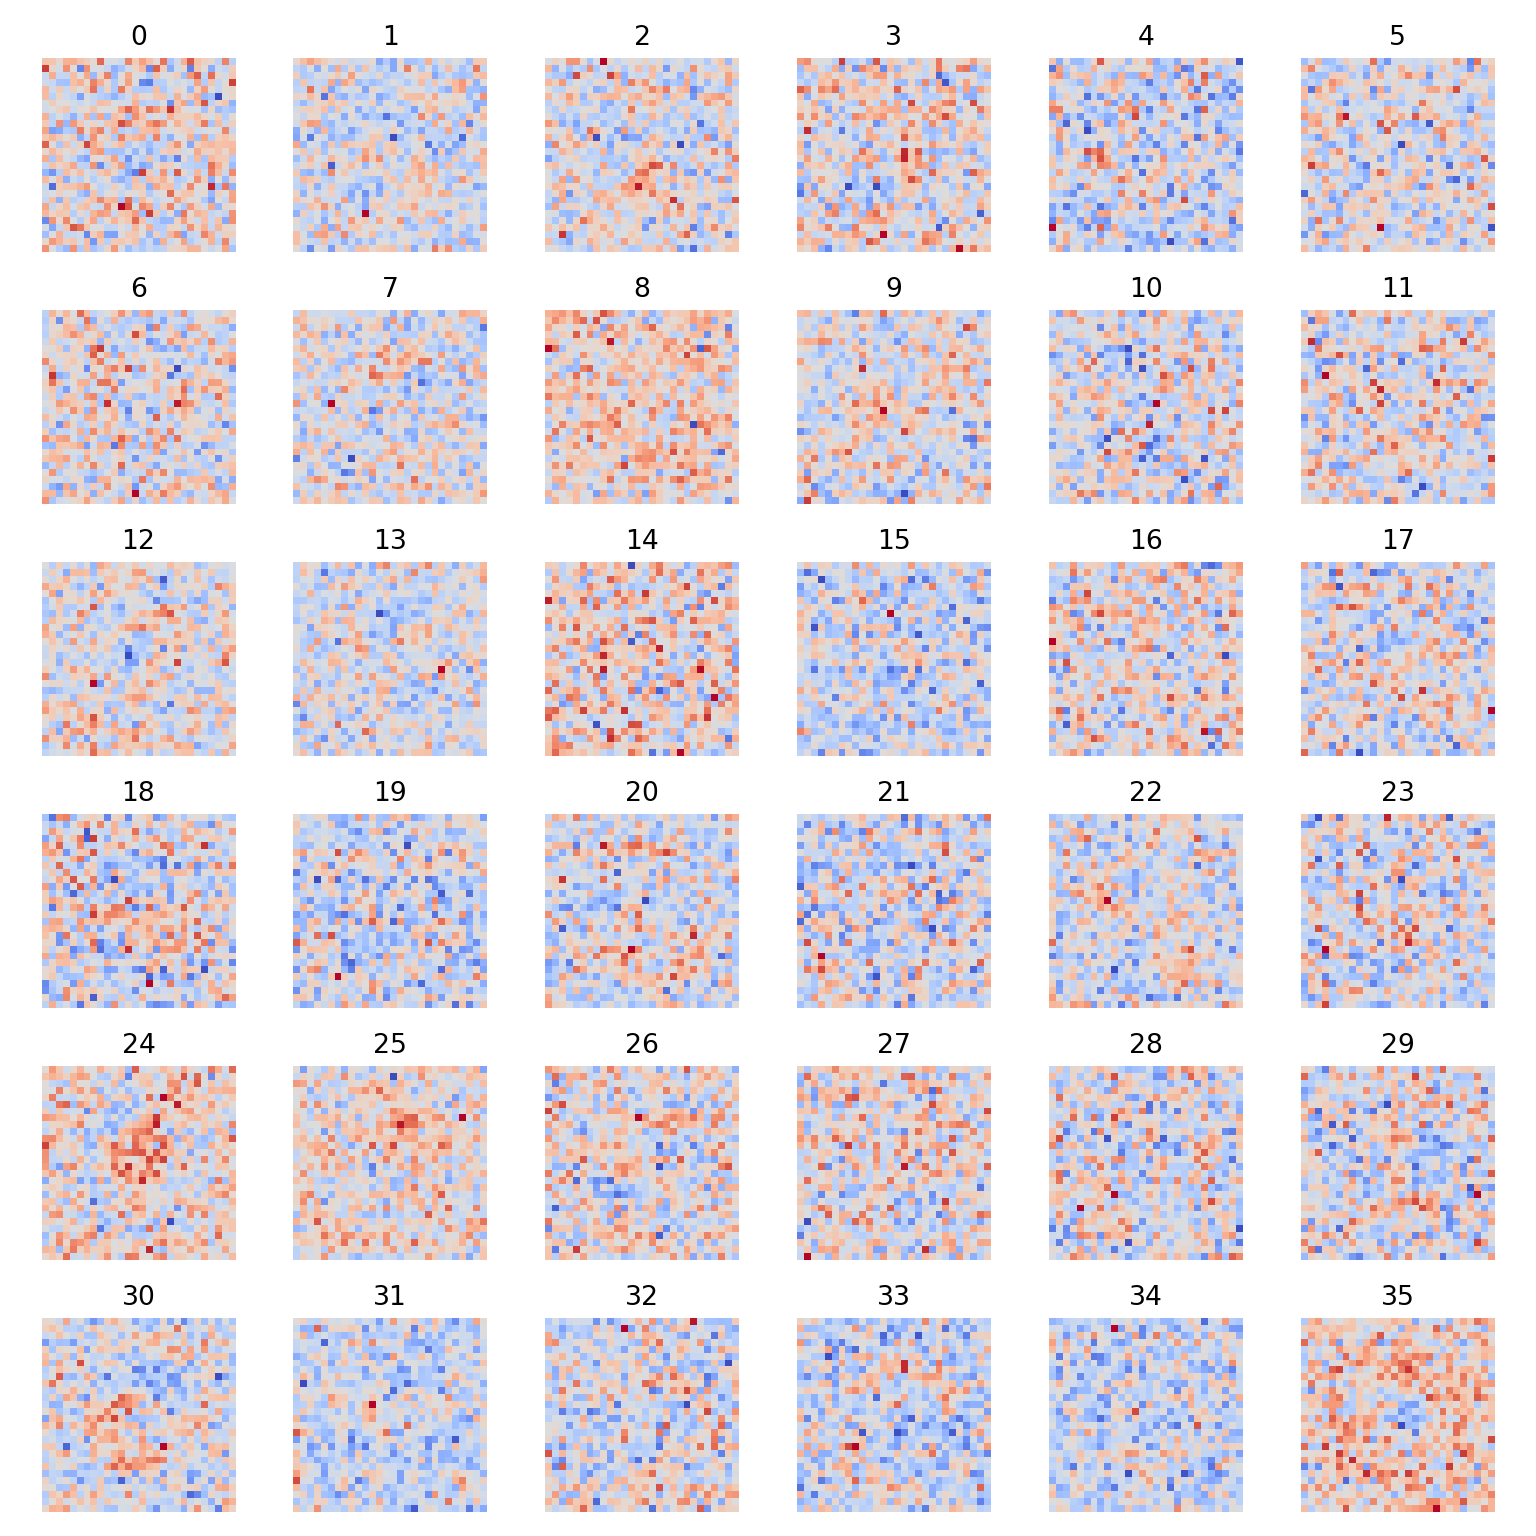
\includegraphics[width=\linewidth]{figures/mlp_first_layer_weights.png}
    \caption{MLP first-layer weights}
  \end{subfigure}
  \begin{subfigure}{0.48\linewidth}
    \centering
    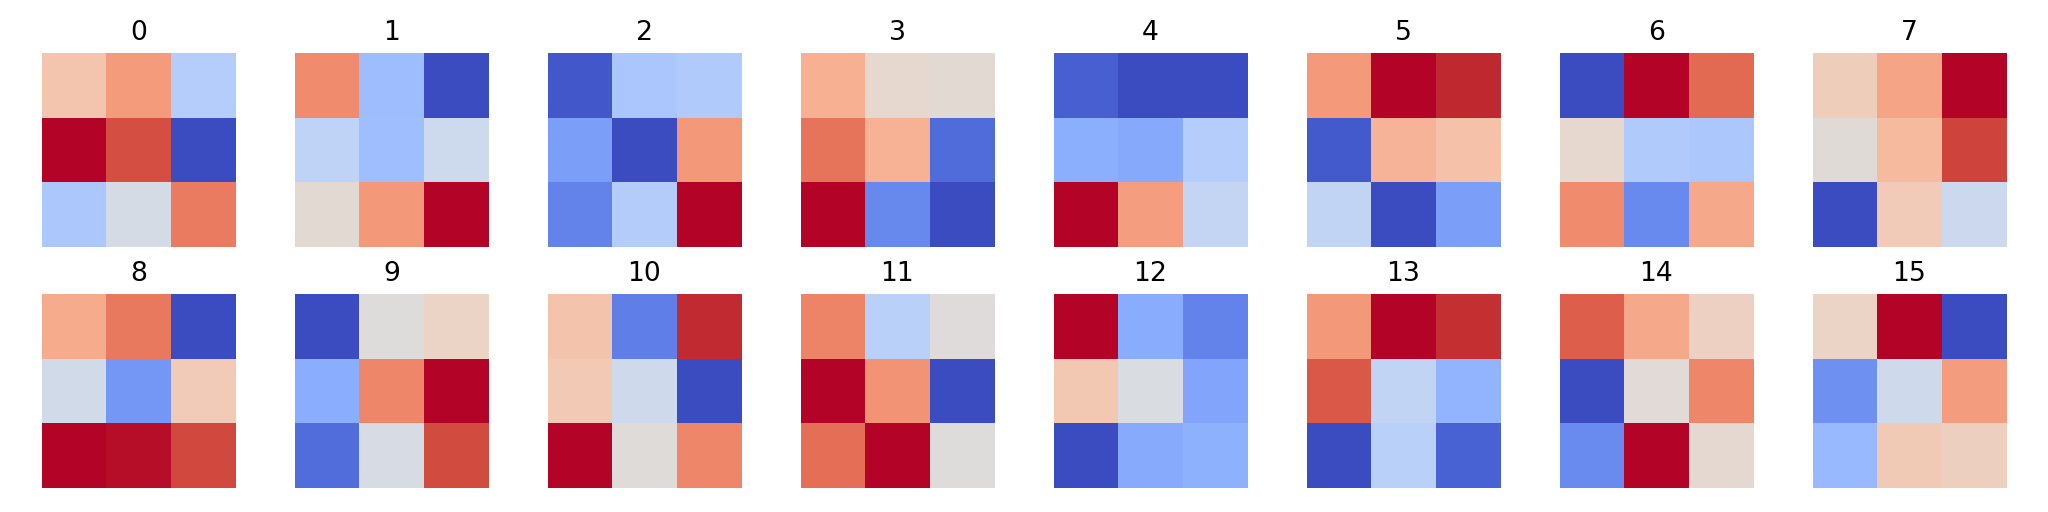
\includegraphics[width=\linewidth]{figures/cnn_kernels.png}
    \caption{CNN convolution kernels}
  \end{subfigure}
  \caption{Model parameter visualizations.}
\end{figure}

\section{Discussion}

The project confirms several expected observations. First, a simple MLP can already solve MNIST reasonably well, reaching 94.59\% test accuracy. Second, optimization matters: changing from SGD to momentum under the same learning rate and scheduler improves MLP test accuracy by 4.42 percentage points. Third, CNNs are better suited for image classification because they exploit local spatial patterns and parameter sharing. After adding max pooling and using the same training setup as the momentum MLP, the CNN reaches 98.46\% test accuracy.

The most informative additional direction is the error analysis. Accuracy alone hides the structure of mistakes. The confusion matrices and misclassified examples show that the hardest cases are not random; they are visually ambiguous digit pairs such as 4/9, 3/5, 2/7, and 5/8. This supports the conclusion that future improvements should target invariance to handwriting style, small deformations, and stroke ambiguity.

\section*{Reproducibility Notes}
All experiments use the provided MNIST dataset only. The fixed random seed is 309. The main scripts are:
\begin{itemize}
  \item \texttt{codes/test\_train.py}: training MLP and CNN models.
  \item \texttt{codes/test\_model.py}: evaluating saved checkpoints.
  \item \path{codes/weight_visualization.py}: confusion matrices, misclassified examples, MLP weights, and CNN kernels.
  \item \texttt{codes/test\_core.py}: unit tests for the implemented operators.
\end{itemize}

\end{document}
